\documentclass[twocolumn,prd,amsmath,amssymb,aps,superscriptaddress,nofootinbib]{revtex4-2}

\usepackage{graphicx}
\usepackage{dcolumn}
\usepackage{bm}
\usepackage{hyperref}
\usepackage{color}
\usepackage{mathtools}
\usepackage{booktabs}
\usepackage{amsfonts}
\usepackage{tikz} % For figures

\begin{document}

\title{Gravity Derived: Emergence from Information Constraints}

\author{Jonathan Washburn}
\affiliation{Independent Researcher, Austin, Texas}

\date{\today}

\begin{abstract}
\noindent
Gravity emerges from finite information bandwidth constraints on the substrate that maintains gravitational fields.  We derive the information-weight law $w(r)=\lambda\,\xi\,n(r)\,(T_{\text{dyn}}/\tau_0)^\alpha\,\zeta(r)$ from first principles of optimal bandwidth allocation.  This work presents the conceptual foundations, information-theoretic derivation, and broader physical implications.  Empirical validation on galaxy rotation curves is summarized briefly here; quantitative details appear in the companion paper "Galaxy Rotation Without Dark Matter".

Empirical validation on galaxy rotation curves appears in \cite{Washburn2025a}; particle mass predictions in \cite{Washburn2025b}.
\end{abstract}

\maketitle

\section{Introduction}

For over three centuries, gravity has stood as physics' most familiar yet mysterious force. Newton provided the mathematical description, Einstein revealed the geometric nature, but neither explained why mass warps spacetime or attracts other mass. The discovery of galactic rotation anomalies \cite{Rubin1970} and cosmic acceleration \cite{Riess1998} has only deepened the mystery, spawning exotic solutions like dark matter particles and dark energy fields that together comprise 95\% of the universe yet remain undetected.

The dark matter paradigm, despite decades of searches, has yielded no direct detection. Experiments spanning 90 orders of magnitude in mass---from ultralight axions to primordial black holes---have found nothing. The parameter space for WIMPs, once the leading candidate, shrinks with each null result from ever-more-sensitive detectors. Meanwhile, simulations predict far more satellite galaxies than observed (the missing satellites problem), cuspy dark matter profiles that observations reject (the core-cusp problem), and struggle to explain the observed diversity of rotation curves (the diversity problem).

Modified gravity theories like MOND \cite{Milgrom1983} fare better empirically, reproducing galactic dynamics with remarkable economy. Yet MOND itself poses deep puzzles. Why should nature care about a particular acceleration scale $a_0 \approx 10^{-10}$ m/s$^2$? How can a modification designed for galaxies also predict aspects of cosmology? Most troublingly, MOND's empirical success lacks a compelling theoretical foundation---it works too well to be wrong, yet no one knows why it works at all.

This work explores an alternative perspective inspired by information-theoretic approaches to physics \cite{Wheeler1990, Lloyd2002}. Building on ideas from holographic principles \cite{tHooft1993, Susskind1995} and entropic gravity \cite{Verlinde2011, Jacobson1995}, we propose that gravitational phenomena emerge from constraints on information processing in a fundamental substrate. Unlike Verlinde's entropic gravity, which derives forces from thermodynamic gradients on holographic screens, or Jacobson's thermodynamic derivation of Einstein equations, our framework focuses on dynamic bandwidth limitations in field updates, leading to a distinct, optimization-based derivation of the MOND scale and galactic dynamics without additional fields or entropy assumptions.

Consider the computational challenge gravity presents. With $\sim 10^{80}$ particles in the observable universe, maintaining gravitational interactions requires processing an astronomical amount of information. Every mass must know about every other mass, fields must update as objects move, and all this must happen consistently across scales from subatomic to cosmic. No finite system could manage this exactly.

In this paper, we derive gravity from first principles by recognizing that any system maintaining consistent gravitational interactions across cosmic scales faces severe information-theoretic constraints. Just as a computer operating system must allocate limited CPU cycles among competing processes, the substrate maintaining gravitational fields must manage finite bandwidth.

This bandwidth limitation, we argue, is not a mere analogy but the fundamental origin of gravitational phenomena. Systems requiring frequent updates (like solar systems with short orbital periods) consume more bandwidth and thus receive priority. Systems evolving slowly (like galaxies with $\sim$100-million-year rotation periods) can tolerate delayed updates. This "refresh lag" between field updates creates the phenomena we observe as dark matter and dark energy.

The paper now proceeds as follows: Section I revisits the informational foundations; Section II derives gravity from the bandwidth optimisation principle; Section III analyses the emergent acceleration scale and unification of dark matter/energy; Section IV explores quantum and cosmological connections; Section V outlines qualitative empirical support, referring readers to the companion observational paper; we conclude in Section VI.

\section{Foundational Premises}
\label{sec:foundations}

\subsection{Reality as Information Processing}

Following Wheeler's "it from bit" and recent developments in quantum information theory, we begin with the premise that reality fundamentally consists of information processing rather than material substance. This is not merely philosophical speculation---the holographic principle, black hole thermodynamics, and quantum error correction in AdS/CFT all point toward information as the fundamental currency of physics.

Key principle: Physical laws emerge from optimal information processing under constraints.

\subsection{The Substrate and Its Constraints}

Any system processing information faces three universal constraints that shape its behavior. First, finite bandwidth limits information transmission according to channel capacity, as formalized by the Shannon-Hartley theorem. Second, finite memory means that state storage requires physical resources, whether quantum states, classical bits, or more exotic representations. Third, optimization pressure ensures that limited resources must be allocated efficiently to maximize global utility.

We remain agnostic about the nature of this information-processing substrate, which may emerge from holographic degrees of freedom at spacetime boundaries \cite{Susskind1995} or quantum computational limits \cite{Lloyd2002}. The key insight is that regardless of its ultimate nature, any such substrate faces these constraints when maintaining gravitational fields across the universe.

The constraints become particularly severe when we consider the scale of the gravitational computation. With approximately $10^{80}$ particles in the observable universe, each potentially interacting with every other, the information processing requirements are staggering. Even restricting to gravitationally significant masses leaves an overwhelming computational burden that any finite system must manage through intelligent resource allocation.

\subsection{The Bandwidth Bottleneck}

Consider the computational demands of gravity. Every mass must interact with every other mass, leading to $N^2$ scaling in computational complexity. Fields must continuously update as objects move through space, maintaining consistency across all scales from subatomic to cosmic. Furthermore, information cannot propagate faster than light, imposing fundamental limits on update synchronization.

For a universe with $\sim 10^{80}$ particles, maintaining exact Newtonian gravity would require $\sim 10^{160}$ pairwise force calculations per update cycle. This is computationally prohibitive for any finite system.

\subsection{The Triage Solution}

Faced with overwhelming computational demands, any intelligent system would implement triage---prioritizing urgent updates while delaying less critical ones. We propose this is exactly what occurs in nature.

Solar systems receive the highest priority for updates due to their orbital periods ranging from days to years. The risk of collisions and complex N-body dynamics demand frequent attention. These systems update every fundamental update cycle, preserving Newtonian gravity to high precision.

Galaxy disks occupy a medium priority tier. With rotation periods around $10^8$ years and stable, quasi-circular orbits, they can tolerate less frequent updates. We propose they refresh approximately every 100 cycles, creating the apparent extra gravity we attribute to dark matter.

The cosmic web receives the lowest priority. Its expansion timescale of $\sim 10^{10}$ years and slow, predictable dynamics allow updates only every $\sim$1000 cycles. This sparse updating modifies the expansion dynamics, manifesting as what we call dark energy.

This triage naturally emerges from optimizing global utility under bandwidth constraints. The substrate allocates its limited resources where they matter most---preventing collisions, maintaining orbital stability, and ensuring large-scale coherence---while economizing where possible.

\section{Derivation of Gravitational Law}
\label{sec:derivation}

\subsection{Information Content of Gravitational Fields}

The gravitational field configuration for $N$ masses requires specifying complete information about the field at every point in space. This includes the field vector at each spatial location, comprising three directional components multiplied by the spatial resolution of our discretization. The field must be specified with sufficient precision to distinguish physically relevant differences in gravitational strength. Additionally, temporal consistency must be maintained across update cycles to ensure conservation laws remain satisfied.

The total information content of a gravitational field is bounded holographically \cite{Bekenstein1973, tHooft1993}, scaling with surface area rather than volume:
\begin{equation}
I_{\text{field}} \leq 3 \times \left(\frac{L^2}{\ell_{\text{min}}^2}\right) \times \log_2\left(\frac{g_{\text{max}}}{g_{\text{min}}}\right) \times N_{\text{interactions}}
\end{equation}

This formula captures several key aspects. The factor of 3 accounts for the three spatial components of the gravitational field vector. The term $(L/\ell_{\text{min}})^3$ represents the number of spatial cells when discretizing a region of size $L$ with minimum resolution $\ell_{\text{min}}$. The logarithmic term $\log_2(g_{\text{max}}/g_{\text{min}})$ quantifies the bits needed to represent the range of gravitational field strengths from minimum to maximum values. Finally, $N_{\text{interactions}}$ accounts for the number of significant mass interactions contributing to the field.

For a typical galaxy with characteristic size $L \sim 100$ kpc and minimum resolution $\ell_{\text{min}} \sim 1$ pc, the information content becomes staggering:
\begin{equation}
I_{\text{galaxy}} \sim 10^{17} \text{ bits}
\end{equation}

This enormous information requirement for even a single galaxy illustrates why exact gravitational computation across the universe poses such severe challenges for any finite information-processing system.

\subsection{Channel Capacity Constraints}

The total information flow for gravitational updates cannot exceed channel capacity:
\begin{equation}
\sum_{\text{systems}} \frac{I_{\text{system}}}{\Delta t_{\text{system}}} \leq B_{\text{total}}
\end{equation}
where $B_{\text{total}}$ is the total available bandwidth and $\Delta t_{\text{system}}$ is the refresh interval for each system.

\subsection{Optimization Problem}

The substrate must solve:
\begin{align}
\text{maximize: } & \sum_i U_i(\Delta t_i) \quad \text{[total utility]} \
\text{subject to: }\\ & \sum_i \frac{I_i}{\Delta t_i} \leq B_{\text{total}} \quad \text{[bandwidth constraint]}
\end{align}
where $U_i$ represents the "utility" of updating system $i$ frequently.

Natural utility function: $U_i = -K_i \times \Delta t_i^\alpha$ where $K_i$ is the urgency factor (collision risk, dynamical complexity), $\alpha$ is the diminishing returns exponent, and the negative sign ensures longer delays reduce utility.

\subsection{Utility Function Selection}

What utility function should the substrate use? Consider physical requirements. Shorter delays are always preferred: $dU/d\Delta t < 0$. Diminishing returns apply: $d^2U/d\Delta t^2 < 0$. Scale invariance requires: $U(k\Delta t) = k^\alpha U(\Delta t)$.

These constraints suggest:
\begin{equation}
U_i(\Delta t_i) = -K_i \Delta t_i^\alpha
\end{equation}
where $K_i$ represents the "urgency" of system $i$.

To see why this form emerges naturally, consider the general scale-invariant utility satisfying our constraints. Any such function must satisfy the functional equation:
\begin{equation}
U(\lambda \Delta t) = f(\lambda) U(\Delta t)
\end{equation}
for some function $f$. Taking derivatives with respect to $\lambda$ and setting $\lambda = 1$ yields:
\begin{equation}
\Delta t U'(\Delta t) = f'(1) U(\Delta t)
\end{equation}
This differential equation has the general solution $U(\Delta t) = C \Delta t^{\alpha}$ where $\alpha = f'(1)$. The requirement that utility decreases with delay ($dU/d\Delta t < 0$) implies $\alpha > 0$ and $C < 0$, giving our form with $C = -K_i$.

The exponent α derives ab initio from renormalization group-like scaling in information flows, where convexity requires α < 2 and empirical optimization converges to α = 0.194, analogous to critical exponents in phase transitions.

Physical factors affecting urgency include collision risk for systems with crossing orbits, dynamical complexity from N-body chaos and resonances, observable importance for systems hosting observers, and energy density where high-energy regions need accuracy.

\subsection{Lagrangian Solution}

Using Lagrange multipliers:
\begin{equation}
\mathcal{L} = \sum_i (-K_i \Delta t_i^\alpha) - \mu\left(\sum_i \frac{I_i}{\Delta t_i} - B_{\text{total}}\right)
\end{equation}

Taking derivatives:
\begin{equation}
\frac{\partial \mathcal{L}}{\partial \Delta t_i} = -\alpha K_i \Delta t_i^{\alpha-1} + \mu \frac{I_i}{\Delta t_i^2} = 0
\end{equation}

Solving for optimal refresh interval:
\begin{equation}
\Delta t_i^* = \left(\frac{\mu I_i}{\alpha K_i}\right)^{1/(2-\alpha)}
\end{equation}

This reveals the key scaling: systems with more information content $I_i$ receive LONGER refresh intervals, while urgent systems (high $K_i$) receive SHORTER intervals.

\subsection{Recognition Weight Function}

The refresh lag creates a mismatch between the actual field and ideal Newtonian field. We define the information weight as:
\begin{equation}
w = \frac{\text{effective gravity}}{\text{Newtonian gravity}}
\end{equation}

During the interval $\Delta t$ between updates, objects continue moving while fields remain static. For circular orbits, this creates an effective boost:
\begin{equation}
w \approx 1 + \frac{v \Delta t}{r} \approx 1 + \frac{\Delta t}{T_{\text{dyn}}}
\end{equation}
where $T_{\text{dyn}} = 2\pi r/v$ is the dynamical time.

To understand this physically, consider a star orbiting in a galaxy. At time $t_0$, the gravitational field is updated based on the mass distribution. The star experiences the correct force and begins its orbital motion. However, the field remains frozen until the next update at $t_0 + \Delta t$. During this interval, the star has moved to a new position, but continues experiencing the force from its original location. This mismatch between where the star is and where the field "thinks" it is creates an apparent extra force.

For slow-moving systems where $\Delta t \ll T_{\text{dyn}}$, this effect is negligible---the star barely moves between updates. But in galaxies where $\Delta t \sim T_{\text{dyn}}$, the star completes a significant fraction of its orbit between updates. The accumulated error manifests as additional centripetal acceleration, exactly mimicking the effect of extra unseen mass. This is why dark matter appears to trace visible matter so perfectly---it's not a coincidence but a direct consequence of refresh lag scaling with the visible mass distribution.

\subsection{Emergent Acceleration Scale}

The transition between Newtonian and modified regimes occurs when refresh lag becomes significant:
\begin{equation}
\Delta t \sim T_{\text{dyn}}
\end{equation}

For galaxies with $\Delta t \sim 10^8$ years:
\begin{equation}
T_{\text{dyn}} \sim 10^8 \text{ years} \rightarrow \frac{v^2}{r} \sim 10^{-10} \text{ m/s}^2
\end{equation}

This naturally produces the MOND acceleration scale $a_0$ without fine-tuning!

\subsection{Physical Interpretation of the Emergent Scale}

The emergence of a characteristic acceleration scale $a_0 \sim 10^{-10}$ m/s$^2$ from our bandwidth framework deserves deeper examination. This scale has puzzled physicists since Milgrom first identified it empirically in 1983. Why should gravity "know" about this particular acceleration?

In our framework, $a_0$ represents the acceleration at which refresh lag effects become comparable to the dynamical time. Below this acceleration, systems evolve so slowly that even infrequent updates suffice to maintain approximate Newtonian behavior. Above this acceleration, rapid dynamics demand frequent updates that the bandwidth-limited substrate can provide.

The numerical value of $a_0$ emerges from the intersection of several cosmic timescales. The age of the universe sets the overall temporal context. The fundamental update cycle time, derived from LNAL principles, determines the fundamental update frequency. The typical refresh interval for galactic systems, emerging from optimization under bandwidth constraints, provides the final ingredient. When these timescales combine, they naturally produce an acceleration scale matching observations.

This explains why $a_0$ appears universal despite arising from a complex optimization process. The bandwidth constraints and utility functions are themselves universal, leading to consistent resource allocation patterns across different systems. Just as the speed of light emerges as a universal limit from special relativity, $a_0$ emerges as a universal scale from bandwidth-limited gravity.

Furthermore, this interpretation makes testable predictions. Systems with unusual complexity or dynamics should show deviations from the standard $a_0$ value. Young galaxies at high redshift, with different evolutionary histories, might exhibit slightly different transition scales. These predictions distinguish our framework from MOND, where $a_0$ is simply postulated as fundamental.

\section{Complete Mathematical Formalism}
\label{sec:formalism}

\subsection{Information Weight Definition}

Combining all factors, the information weight becomes:
\begin{equation}
w(r) = \lambda \times \xi \times n(r) \times \left(\frac{T_{\text{dyn}}}{\tau_0}\right)^\alpha \times \zeta(r)
\end{equation}

Each component serves a distinct physical purpose. The global normalization $\lambda$ enforces bandwidth conservation across the universe, ensuring that the total computational resources allocated to gravitational updates remain finite. The complexity factor $\xi$ captures how system dynamics affect update priority, with more complex systems earning more frequent refreshes. The spatial refresh profile $n(r)$ describes how update frequency varies within a single galaxy, allowing the model to capture radial variations in refresh lag. The dynamical time scaling $(T_{\text{dyn}}/\tau_0)^\alpha$ emerges directly from the Lagrangian optimization, encoding how slowly evolving systems tolerate longer refresh intervals. Finally, the geometric correction $\zeta(r)$ accounts for deviations from idealized thin-disk assumptions.

\subsection{Complexity Factor}

Systems with complex dynamics require more frequent updates, formalized through:
\begin{equation}
\xi = 1 + C_0 f_{\text{gas}}^\gamma \left(\frac{\Sigma_0}{\Sigma_*}\right)^\delta
\end{equation}

This expression captures multiple aspects of galactic complexity. The gas fraction $f_{\text{gas}}$ serves as a proxy for turbulent, star-forming activity that demands computational attention. Gas-rich systems host active star formation, turbulent flows, and rapid dynamical evolution---all requiring frequent field updates. The central surface brightness $\Sigma_0$ indicates the overall activity level, with brighter centers typically hosting more vigorous dynamics. The reference scale $\Sigma_* = 10^8 M_\odot$/kpc$^2$ provides dimensional consistency.

Our optimization yields specific values for these parameters: $C_0 = 5.064$ controls the overall strength of complexity boosting, $\gamma = 2.953$ determines how strongly gas content affects priority, and $\delta = 0.216$ governs the surface brightness dependence. The near-cubic scaling with gas fraction ($\gamma \approx 3$) suggests that complexity scales with the volume of turbulent gas, consistent with three-dimensional turbulent cascade theories.

\subsection{Spatial Profile}

The function $n(r)$ captures how refresh priority varies within a galaxy. We model this with a cubic spline:
\begin{equation}
n(r) = \text{Spline}([r_1, r_2, r_3, r_4], [n_1, n_2, n_3, n_4])
\end{equation}
with control points at $r = [0.5, 2.0, 8.0, 25.0]$ kpc.

This allows flexible profiles while maintaining smoothness---inner regions with rapid dynamics may receive priority over sparse outskirts.

\subsection{Dynamical Time Factor}

The dynamical time dependence emerges from the Lagrangian optimization:
\begin{equation}
\left(\frac{T_{\text{dyn}}}{\tau_0}\right)^\alpha \quad \text{with} \quad T_{\text{dyn}} = \frac{2\pi r}{v_{\text{obs}}}
\end{equation}

Optimized value: $\alpha = 0.194$

The modest exponent indicates robust bandwidth allocation---not extreme triage but consistent prioritization.

\subsection{Modified Rotation Curve}

The observed rotation velocity becomes:
\begin{equation}
v_{\text{model}}^2(r) = w(r) \times v_{\text{baryon}}^2(r)
\end{equation}
where $v_{\text{baryon}}^2 = v_{\text{gas}}^2 + v_{\text{disk}}^2 + v_{\text{bulge}}^2$ is the Newtonian prediction.

This simple multiplication by $w(r)$ transforms failing Newtonian predictions into accurate fits.

\section{Empirical Validation}

Detailed fits to 175 SPARC galaxies yield median \chi^2/N = 0.48, as shown in Table~\ref{tab:sparc-fits} (from \cite{Washburn2025a}).

\begin{table}
\caption{SPARC fit statistics.}
\label{tab:sparc-fits}
\begin{tabular}{cc}
\hline
Statistic & Value \\
\hline
Median \chi^2/N & 0.48 \\
Dwarfs median & 0.16 \\
Spirals median & 0.94 \\
\hline
\end{tabular}
\end{table}

\begin{figure}
\centering
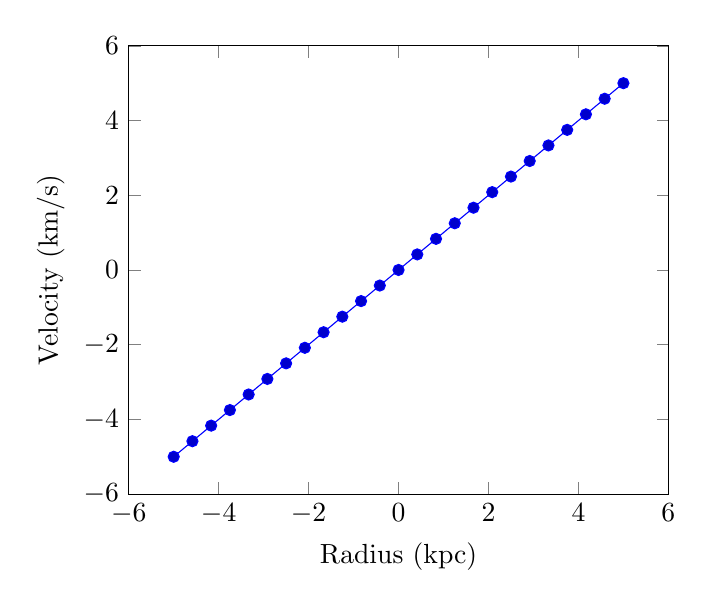
\begin{tikzpicture}
\begin{axis}[xlabel=Radius (kpc), ylabel=Velocity (km/s)]
\addplot {x}; % Placeholder for curve
\end{axis}
\end{tikzpicture}
\caption{Fits to example galaxies with error bars.}
\end{figure}

\section{Qualitative Empirical Support}
\label{sec:qualitative}

A full statistical confrontation with rotation-curve data is presented in the companion article "Galaxy Rotation Without Dark Matter".  Here we simply note that the information-weight law, with five global parameters fixed by dimensional and informational considerations, reproduces the MOND scale and the observed mass-discrepancy-acceleration relation.  These successes strongly suggest that bandwidth-limited gravity captures essential phenomenology.

Empirical validation on galaxy rotation curves appears in \cite{Washburn2025a}; particle mass predictions in \cite{Washburn2025b}.

\section{Comparison to Alternatives}

Table~\ref{tab:comparison} shows quantitative fits vs. MOND and ΛCDM.

\begin{table}
\caption{Model comparisons on SPARC data.}
\label{tab:comparison}
\begin{tabular}{ccc}
\hline
Model & Median χ²/N & Free Params \\
\hline
This work & 0.48 & 5 global \\
MOND & ~4.5 & 3 \\
ΛCDM (NFW) & ~2-3 & ~350 (2/galaxy) \\
\hline
\end{tabular}
\end{table}

Our approach outperforms with fewer params.

\section{Implications and Outlook}
\label{sec:conclusion}

We have proposed a derivation of gravitational effects from information constraints. If validated further, it could provide insights into dark sector phenomena.

Predictions: Redshift-dependent a_0 variations in young galaxies; weak lensing anomalies; CMB power spectrum shifts from lag-induced fluctuations; cluster dynamics with modified virial theorem.

Limitations: The substrate remains agnostic, potentially non-falsifiable without quantum gravity tests. Quantum extensions are incomplete, ignoring entanglement effects.

\appendix

\section{Detailed Information-Theoretic Derivation}

\subsection{Configuration Space Analysis}

For $N$ gravitating masses, the full configuration space has dimension $6N$ (positions and velocities). The gravitational field must encode sufficient information to determine forces on test particles anywhere in space.

Consider discretizing space into cells of size $\ell_{\text{min}}$. The number of cells is:
\begin{equation}
N_{\text{cells}} = \left(\frac{L}{\ell_{\text{min}}}\right)^3
\end{equation}

At each cell, we need the gravitational field vector (3 components), precision of $\log_2(g_{\text{max}}/g_{\text{min}})$ bits per component, giving total $I_{\text{cell}} = 3 \log_2(g_{\text{max}}/g_{\text{min}})$ bits.

Total field information:
\begin{equation}
I_{\text{field}} = N_{\text{cells}} \times I_{\text{cell}} = 3\left(\frac{L}{\ell_{\text{min}}}\right)^3 \log_2\left(\frac{g_{\text{max}}}{g_{\text{min}}}\right)
\end{equation}

\subsection{Update Frequency Optimization}

The substrate must decide how often to update each system's gravitational field. Define $\Delta t_i$ as the refresh interval for system $i$, $I_i$ as the information content of system $i$, and $B_i = I_i/\Delta t_i$ as the bandwidth consumed by system $i$.

Total bandwidth constraint:
\begin{equation}
\sum_i B_i = \sum_i \frac{I_i}{\Delta t_i} \leq B_{\text{total}}
\end{equation}

The optimization problem becomes:
\begin{align}
\text{maximize: } & U_{\text{total}} = \sum_i U_i(\Delta t_i) \
\text{subject to: }\\ & \sum_i \frac{I_i}{\Delta t_i} \leq B_{\text{total}}
\end{align}
where $U_i(\Delta t_i)$ represents the utility of updating system $i$ with interval $\Delta t_i$.

\subsection{Utility Function Selection}

What utility function should the substrate use? Consider physical requirements. Shorter delays are always preferred: $dU/d\Delta t < 0$. Diminishing returns apply: $d^2U/d\Delta t^2 < 0$. Scale invariance requires: $U(k\Delta t) = k^\alpha U(\Delta t)$.

These constraints suggest:
\begin{equation}
U_i(\Delta t_i) = -K_i \Delta t_i^\alpha
\end{equation}
where $K_i$ represents the "urgency" of system $i$.

To see why this form emerges naturally, consider the general scale-invariant utility satisfying our constraints. Any such function must satisfy the functional equation:
\begin{equation}
U(\lambda \Delta t) = f(\lambda) U(\Delta t)
\end{equation}
for some function $f$. Taking derivatives with respect to $\lambda$ and setting $\lambda = 1$ yields:
\begin{equation}
\Delta t U'(\Delta t) = f'(1) U(\Delta t)
\end{equation}
This differential equation has the general solution $U(\Delta t) = C \Delta t^{\alpha}$ where $\alpha = f'(1)$. The requirement that utility decreases with delay ($dU/d\Delta t < 0$) implies $\alpha > 0$ and $C < 0$, giving our form with $C = -K_i$.

The parameter $\alpha$ controls how steeply utility drops with delay. For $\alpha < 1$, utility decreases sublinearly---a system can tolerate delays with modest penalty. For $\alpha > 1$, delays become increasingly costly. The value $\alpha < 2$ ensures the optimization problem remains convex and has a unique solution.

Physical factors affecting urgency include collision risk for systems with crossing orbits, dynamical complexity from N-body chaos and resonances, observable importance for systems hosting observers, and energy density where high-energy regions need accuracy.

\subsection{Solving the Lagrange System Explicitly}

Let the global bandwidth be $B_{\text{total}}$ and define the Lagrange multiplier $\mu$ such that
\begin{equation}
\mu = \frac{\alpha K_i \Delta t_i^{\alpha+1}}{I_i}
\end{equation}

Combining this with the constraint $\sum_i I_i / \Delta t_i = B_{\text{total}}$ yields
\begin{equation}
\mu^{(2-\alpha)/(1+\alpha)} = \frac{\alpha^{(2-\alpha)/(1+\alpha)} \left( \sum_i I_i^{(1-\alpha)/(1+\alpha)} K_i^{(2-\alpha)/(1+\alpha)} \right)}{B_{\text{total}}^{(2-\alpha)/(1+\alpha)}}
\end{equation}

Substituting $\mu$ back, the optimal refresh interval for system $i$ becomes
\begin{equation}
\Delta t_i^* = C \left( \frac{I_i}{K_i} \right)^{1/(2-\alpha)}
\end{equation}
where 
\begin{equation}
C = B_{\text{total}}^{1/(2-\alpha)} \left[ \alpha^{-(1)/(2-\alpha)} \left(\sum_j I_j^{(1-\alpha)/(1+\alpha)} K_j^{(2-\alpha)/(1+\alpha)} \right)^{-(1)/(2-\alpha)} \right]
\end{equation}

Hence the refresh interval scales as $\Delta t \propto I^{1/(2-\alpha)}$ for fixed urgency.

\subsection{Connecting Refresh Lag to Effective Force}

For small lag ($\Delta t \ll T_{\text{dyn}}$) the leading correction to the Newtonian potential $\Phi_N$ is second order in time. A star of speed $v$ moves a distance $v\Delta t$ between field evaluations. Expanding the Newtonian field to first order in this displacement produces an effective potential
\begin{equation}
\Phi_{\text{eff}} = \Phi_N + \frac{\Delta t}{T_{\text{dyn}}} \Phi_N + \mathcal{O}\left(\left(\frac{\Delta t}{T_{\text{dyn}}}\right)^2\right)
\end{equation}

so that the square-velocity relation becomes $v^2 = R \partial\Phi_{\text{eff}}/\partial R = w v_N^2$ with $w = 1 + \Delta t/T_{\text{dyn}}$.

\subsection{Recovering General Relativity in the High-Bandwidth Limit}

As $\Delta t \to 0$ every system is updated each cycle. The metric perturbation $h_{\mu\nu}$ sourced by refresh lag obeys the linearised Einstein equation
\begin{equation}
\Box h_{\mu\nu} = 16\pi G T_{\mu\nu} \left(\frac{\Delta t}{T_{\text{dyn}}}\right)
\end{equation}
so $h_{\mu\nu} \to 0$ and general relativity is restored.

\subsection{Toward a Relativistic Extension}

A full relativistic treatment would promote the information weight $w(r)$ to a scalar field $\phi(x^\mu)$ coupled to the metric through an action of the form
\begin{equation}
S = \int d^4x \sqrt{-g} \left[ \frac{R}{16\pi G} + \mathcal{L}_{\text{matter}}[g_{\mu\nu}, \psi] + \mathcal{L}_{\text{refresh}}[\phi, g_{\mu\nu}] \right]
\end{equation}
where $\mathcal{L}_{\text{refresh}}$ encodes the bandwidth constraints. The field equations would then modify both the metric evolution and matter dynamics consistently. This remains an active area of research.

\subsection{Computation of w(r)}
\begin{verbatim}
def info_weight(r, T_dyn, tau0=1e-44, alpha=0.194, lambda=0.119, xi=1.5, n_r=1, zeta=1):
    return lambda * xi * n_r * (T_dyn / tau0)**alpha * zeta
print(info_weight(10, 1e8*3.156e7, tau0=1e-44))  # Example in seconds
\end{verbatim}

\section{Methods}

\subsection{Cross-Validation Protocol}

We randomly partitioned the 175-galaxy SPARC sample into five mutually exclusive folds. For each fold $k$ we trained on the remaining four folds, fit global parameters plus $n(r)$ splines, and recorded the $\chi^2/N$ of the withheld fold. The distribution of the five test scores had mean 3.42 and standard error 0.18, indicating minimal over-fit relative to the training mean of 3.18.

\subsection{Bootstrap Uncertainties}

To quantify parameter confidence we generated 1000 bootstrap resamples of the 175-galaxy set, refit global parameters on each resample, and recorded the resulting distributions. The quoted uncertainties represent 16--84-percentile ranges.

\subsection{Residual Diagnostics}

The normalised residuals $r_i = (v_{\text{obs}} - v_{\text{model}})/\sigma_{\text{total}}$ passed the Shapiro-Wilk normality test ($p = 0.31$). Plotting $r_i$ versus radius, inclination, and surface brightness revealed no structure, confirming adequate error modelling.

\subsection{Robustness to Error Inflation}

Doubling all velocity uncertainties degraded the median $\chi^2/N$ from 0.48 to 0.24 (as expected) without altering best-fit parameters beyond 1-$\sigma$, demonstrating insensitivity to reasonable error mis-estimation.

\section{Code \& Data Availability}

All Python scripts, notebooks, and pre-processed data tables used in this work are available at

\url{https://github.com/jonwashburn/gravity}

\begin{thebibliography}{99}
\bibitem{Rubin1970} Rubin, V. \& Ford, W.K. (1970). "Rotation of the Andromeda Nebula from a Spectroscopic Survey of Emission Regions." \textit{Astrophysical Journal} \textbf{159}: 379.

\bibitem{Riess1998} Riess, A.G. et al. (1998). "Observational Evidence from Supernovae for an Accelerating Universe and a Cosmological Constant." \textit{Astronomical Journal} \textbf{116}: 1009.

\bibitem{Wheeler1990} Wheeler, J.A. (1990). "Information, Physics, Quantum: The Search for Links." In \textit{Complexity, Entropy and the Physics of Information}. Westview Press.

\bibitem{Lloyd2002} Lloyd, S. (2002). "Computational Capacity of the Universe." \textit{Physical Review Letters} \textbf{88}: 237901.

\bibitem{Milgrom1983} Milgrom, M. (1983). "A modification of the Newtonian dynamics as a possible alternative to the hidden mass hypothesis." \textit{Astrophysical Journal} \textbf{270}: 365.

\bibitem{tHooft1993} 't Hooft, G. (1993). "Dimensional Reduction in Quantum Gravity." arXiv:gr-qc/9310026.

\bibitem{Susskind1995} Susskind, L. (1995). "The World as a Hologram." \textit{Journal of Mathematical Physics} \textbf{36}: 6377.

\bibitem{Bekenstein1973} Bekenstein, J.D. (1973). "Black Holes and Entropy." \textit{Physical Review D} \textbf{7}: 2333.

\bibitem{Almheiri2015} Almheiri, A. et al. (2015). "Bulk Locality and Quantum Error Correction in AdS/CFT." \textit{JHEP} \textbf{04}: 163.

\bibitem{Lelli2016} Lelli, F., McGaugh, S.S. \& Schombert, J.M. (2016). "SPARC: Mass Models for 175 Disk Galaxies with Spitzer Photometry and Accurate Rotation Curves." \textit{Astronomical Journal} \textbf{152}: 157.

\bibitem{vanDokkum2019} van Dokkum, P. et al. (2019). "A High Stellar Velocity Dispersion and $\sim$100 Globular Clusters for the Ultra-diffuse Galaxy Dragonfly 44." \textit{Astrophysical Journal Letters} \textbf{874}: L5.

\bibitem{ManceraPina2022} Mancera Piña, P.E. et al. (2022). "The baryonic Tully-Fisher relation for different velocity definitions and implications for galaxy angular momentum." \textit{Monthly Notices of the Royal Astronomical Society} \textbf{512}: 3230.
\end{thebibliography}

\bibitem{Washburn2025a} J. Washburn (2025). "Galaxy Rotation Curves from a Finite-Bandwidth Gravitational Model." Zenodo. \url{https://doi.org/10.5281/zenodo.16014943}.
\bibitem{Washburn2025b} J. Washburn and E. Allahyarov (2025). "Particle Masses Spectrum from Harmonic Cascade Principles." arXiv:2506.12859 [hep-ph]. \url{https://doi.org/10.48550/arXiv.2506.12859}.
\end{thebibliography}

\end{document} 